\documentclass[conference]{IEEEtran}
\IEEEoverridecommandlockouts
% The preceding line is only needed to identify funding in the first footnote. If that is unneeded, please comment it out.
\usepackage{cite}
\usepackage{amsmath,amssymb,amsfonts}
\usepackage{algorithmic}
\usepackage{enumitem}
\usepackage{graphicx}
\usepackage{textcomp}
\usepackage{xcolor}
\def\BibTeX{{\rm B\kern-.05em{\sc i\kern-.025em b}\kern-.08em
    T\kern-.1667em\lower.7ex\hbox{E}\kern-.125emX}}
\graphicspath{{Figures/}}
\usepackage[normalem]{ulem}

\begin{document}

\title{Secure Industrial Control System with Intrusion Detection
% {\footnotesize \textsuperscript{*}Note: Sub-titles are not captured in Xplore and
% should not be used}
}

\author{\IEEEauthorblockN{M Rayhan Ahmed Mithu, Rajesh Manicavasagam}
\IEEEauthorblockA{\textit{Computer Science Department} \\
\textit{Tennessee Technological University}\\
Cookeville, TN, United States of America \\
mmithu42, rmanicava42@students.tntech.edu}
\and
\IEEEauthorblockN{Michael Rogers, Denis Ulybyshev}
\IEEEauthorblockA{\textit{Computer Science Department, CEROC} \\
\textit{Tennessee Technological University}\\
Cookeville, TN, United States of America \\
mrogers, dulybyshev@tntech.edu}
% \IEEEauthorblockN{3\textsuperscript{rd} Given Name Surname}
% \IEEEauthorblockA{\textit{dept. name of organization (of Aff.)} \\
% \textit{name of organization (of Aff.)}\\
% City, Country \\
% email address}
% \and
% \IEEEauthorblockN{4\textsuperscript{th} Given Name Surname}
% \IEEEauthorblockA{\textit{dept. name of organization (of Aff.)} \\
% \textit{name of organization (of Aff.)}\\
% City, Country \\
% email address}
% \and
% \IEEEauthorblockN{5\textsuperscript{th} Given Name Surname}
% \IEEEauthorblockA{\textit{dept. name of organization (of Aff.)} \\
% \textit{name of organization (of Aff.)}\\
% City, Country \\
% email address}
% \and
% \IEEEauthorblockN{6\textsuperscript{th} Given Name Surname}
% \IEEEauthorblockA{\textit{dept. name of organization (of Aff.)} \\
% \textit{name of organization (of Aff.)}\\
% City, Country \\
% email address}
}

\maketitle

\begin{abstract}
Detecting intrusions and anomalies in Industrial Control Systems at early stages is important to prevent process failure. Detection of intrusion based on network data alone might not be sufficient. Operator errors, device or equipment failures, and other non-network events could lead to a critical state. As a result, these events can indirectly lead to anomalous network traffic, and, thus, the number of false positives and false negatives generated by the intrusion detection system rises. In this paper, we propose a novel approach of using device state information, stored in a secure data container, to improve the detection accuracy. Our methodology allows to detect anomalies as well as their root causes, which is essential. We use a secure data container to store log records for devices in cyber-physical systems. Secure data container provides protection for log records in transit and at rest. Our data container supports role-based and attribute-based access control and protects against insider threats. 
\end{abstract}

\begin{IEEEkeywords}
Data Privacy, Industrial Control Systems, Intrusion Detection, Secure Data Container
\end{IEEEkeywords}

\section{Introduction}
Industrial Control Systems (ICS) automate the manufacturing process. They are responsible for controlling and managing a potentially large number of field devices. The manufacturing industry has seen a huge rise in the adoption of ICS in recent years, and this growth will continue according to the study report published by Market Research Future (MRFR)~\cite{c1}. Many ICS are deployed in critical infrastructures such as the Smart Grid, health care systems, water purification systems, and nuclear plants. As a result, security breaches and attacks can have significant impact on human lives are very costly. Securing these systems has become a priority as a result of the increasing number of attacks in this domain. 
\par Even though many approaches for intrusion detection in ICS are present in the literature, we observe that most of these solutions focus on the network traffic data generated in the ICS. We propose to use device state information along with network data packets to detect intrusions. Consider Figure~\ref{SICSA} which is based on the Purdue Enterprise Reference Architecture~\cite{c11}. If intrusion is detected in a data network on level 2, we query devices at a lower level to check device state related to the network data that caused intrusion alert on a higher level. Our approach verifies the alert generated by an Intrusion Detection System (IDS) by determining whether suspicious network packets that caused the IDS alert are consistent with the state of the lower level devices. Thus, our approach can not only detect the anomaly, but also find the root cause of the anomaly. 

Device state data is stored as log records in a Secure Data Container (SDC), which guarantees confidentiality and integrity of data that is used to detect anomaly root cause. SDC provides data protection in transit and at rest. Data along with access control policies are stored in the SDC in encrypted form. Separate encryption keys, one per data subset, are generated on-the-fly and are not stored inside the SDC or on any Trusted Third Party. SDC supports role-based and attribute-based access control. A Central Authority is not required for recipient key generation or for access control policy enforcement. Furthermore, the SDC protects against insider threats and can detect several types of data leakages.      
\par The rest of the paper is organized as follows. Section II presents an overview of related work. In Section III the core design is presented. Preliminary experimental results are discussed in Section IV. Section V discusses the future work and section VI concludes the paper.  

\section{Related Work}
The following related work focuses on the state of the art of IDS. The IDS is not only a popular software-based solution that is in practical use, but also has been a focus of research in securing ICS.

\par Morris, Vaughn, and Dandass~\cite{c2} proposed an IDS that focuses on devices that are connected with serial links. The authors proposed a Snort-based IDS for MODBUS\textsuperscript{\textregistered} in both a passive mode and an inline mode that dropped packets. 
% {\color{red} MDR: Say what they found - what was the result of their research?  Also, it would be good to state its shortcoming as compared to our work.}
A signature-based IDS with state-based rules and stand alone IDS rules was presented in a later work in \cite{c9}.
\par A critical state analysis-based approach by Carcano et al. \cite{c4} in SCADA systems uses state information to detect intrusion. A software virtual image with software object representing all devices of the monitored system was used to monitor the evolution of system states. The IDS was implemented on the virtual image and an alert was triggered if the current state was critical or moving towards a critical state.

Unfortunately, both of the above mentioned approaches require expert domain knowledge to model normal and critical device state. They also do not address the problem of integrity of the state information from devices which can be attacked. Our approach uses machine learning algorithms to identify important device state information and co-relate it with the network packets. Moreover, we use a secure data container to store the device state information, which provides data privacy and integrity.
\par A multi-agent IDS was proposed by Tsan and Kwong \cite{c3} in industrial network. They implemented the unsupervised Ant Colony Clustering Model (ACCM) in the "decision agent" that is responsible for learning and classification of prepossessed data. This implementation shows the improved performance of ant-based clustering. K-Means clustering achieves 89.17\% average detection rate and  4.29\% false positive rate with the Fast Independent Component Analysis (FastICA) feature extraction. Unfortunately, any false alarms could lead to disastrous consequences.
% {\color{red} MDR: Here is a good time to make a statement about how such false postitives are high.  .}
% {\color{red} MDR: state what is different from our work.  Example: they need domain experts to model device behavior.  These domain experts need to be experts on how the device hardware works, and also experts on the industrial process to understand how the device state can move toward critical states.  However, our approach will require no such domain expertise, but will use machine learning techniques to associate device state with network patterns.  Also point out that they do not not address the problem of the integrity of the device state, which can also be attacked.  We use secure data containers to ensure device state integrity.}

Ranchal et al \cite{c10} proposed EPICS solution for web services to protect data throughout the service interaction lifecycle. This solution expands the Active Bundle concept \cite{c12}, \cite{c13}, \cite{c14} for data protection. Datasets are stored and transferred together with the access control policies and with the data disclosure monitor. Our solution for SDC is similar to an Extended Attribute-Aware Active Bundle \cite{c6} and it expands the Active Bundle concept with the following capabilities: \\
(a) detection of data leakages made by authorized insiders; \\
(b) support of SDC as a spreadsheet file. 

Awad, Lopez, and Rogers~\cite{c8} propose a framework for live memory forensics of level 0-1 devices by continually acquiring portions of volatile memory and monitoring changes.  This work's primary use is for memory forensics, but could be complementary to our work as a source for generating log records.
                                                                            
\section{Core Design}
% \subsection{Industrial Control Systems Security}
%%Industrial control system was initially designed to operate within a close environment and manage the overall system. However, this has changed as the ICS network is now globally connected via the internet technology. The global connection has a lot of benefits that includes managing multiple field sites with thousands of devices in different location from one control center, faster data access and and inseparability among devices with different communication protocols. It also exposed the industrial control system to all the vulnerabilities and security threats that exists in the commercial network.Communication among the main components such as programmable logic controller (PLC), supervisory control and data acquisition (SCADA), Control devices is what makes this whole system functional. The communication protocols for these components are not similar to the typical commercial network protocols. Security was not a big concern when these protocols were designed as the system was kept isolated from the outside world. 
Initially, ICS were designed for local processes isolated from Wide Area Networks (WANs) and, therefore, had little or no security. However, as processes became more complex and business needs grew, providing connectivity to WANs became necessary. 
Unfortunately, the unlimited access of the Internet made the ICS vulnerable to attacks. Furthermore, retrofitting ICS devices with new secure communication protocols is too expensive. In addition, field devices cannot run computationally intensive algorithms due to limited resources. 

%\begin{figure}[htbp]
%\centering
%\centerline{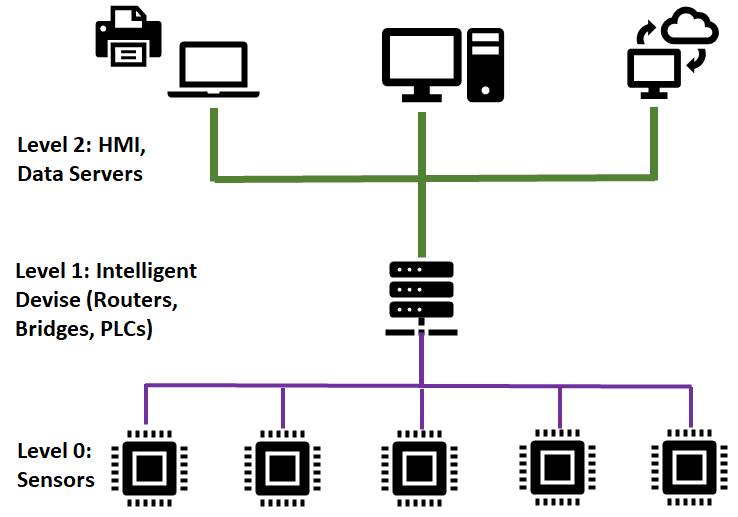
\includegraphics [width=9cm] {ICS-Architecture-RelOK.png}}
%\caption{Industrial Control System Architecture}
%\label{ICS_Arch}
%\end{figure}

Therefore, IDS have become a popular security method for detecting attacks. An IDS can be added to an existing network at a strategic point without needing to modify existing devices.
%Intrusion detection system is a great method for attack detection and prevention in the commercial network by monitoring network traffic with rule based or anomaly based approach. 
However, in the industrial network it is not always enough to monitor the network traffic alone. For example, a sequence of (valid) control commands, device failures, faulty raw materials, etc, could lead to a critical situation in the process.  This critical situation will likely result in unusual network traffic as the control devices attempt to notify the process control personnel. As a result, false positives indicating that the network is being attacked are generated by the IDS.  Believing that a network attack is underway, the process control personnel might not respond correctly to the critical state, which could have disastrous results. 

We propose a novel approach where the IDS can validate network traffic with the help from the device generating the traffic. Log records of device state information are created and stored. The device state information is kept in an SDC which can be accessed upon request. Machine learning algorithms will learn what device state is associated with which network communication patterns, and provide this information as a database to the IDS. The IDS will monitor network patterns and, when an anomaly is suspected, can query SDCs for involved devices, and the database to validate its suspicions. Secure ICS architecture is illustrated in Figure~\ref{SICSA}. 

\begin{figure}[htbp]
\centering
\centerline{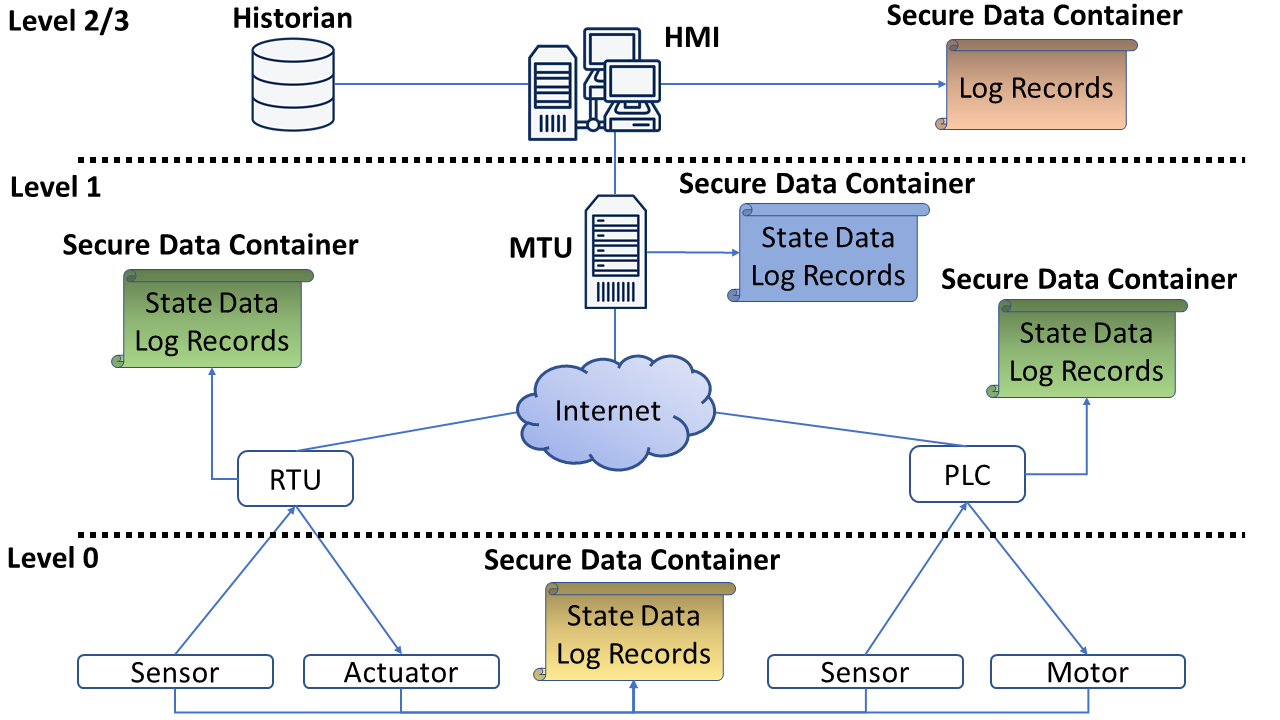
\includegraphics [width=.5\textwidth]{sec_arch.png}}
\caption{Secure Industrial Control System Architecture}
\label{SICSA}
\end{figure}

%%The architecture has four major components:
Secure ICS has five major components, illustrated in Figure~\ref{sec_ics}, that are described as follows.

% {\color{red} Ok, so following is what I think we need to describe:  First, all components feed into the secure data container component.  That component provides a secure mechanism for storing and retrieving data for all the other componenents in the system.  The  Embedded component runs on the SCADA devices and collects device state.  It can do this in a miriad of ways, including sampling, logging. etc.  It produces a log file that is stored in a secure data container.  The State identification module uses log records of state stored in a secure container to produce an image that represents an instantaneous state of the system that likely results in a change in network state.  The training component trains  offline.  Its training accomplishes two goals.  One is learning what state information is most likely to result in significant network traffic pattern changes (this information is used by the state identification module), and the other is learning what device state produces particular network state. So, we need to restructure/rewrite the description below to reflect this.  See my simplistic picture:}
% 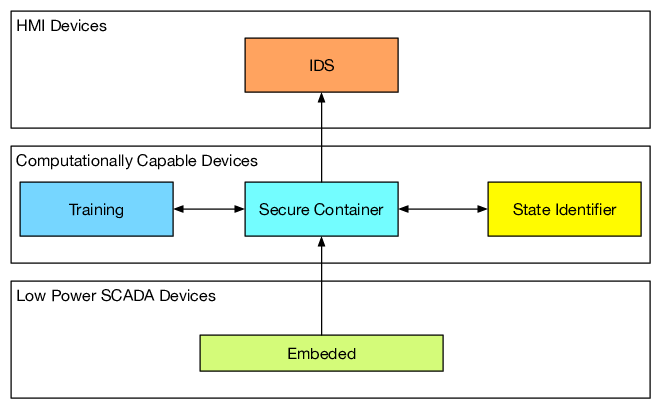
\includegraphics [width=.4\textwidth]{secscada.png}
\subsection{Embedded Components}
The {\em embedded components} of the system will monitor ICS devices in real time, create log records, and transfer the log records to the SDC. Two modules are required to execute these actions. The first module is the \textit{\textbf{State Monitor}} and the other module is called \textit{\textbf{State Router}}. The state monitor module is responsible for real time monitoring of the device state. It can collect device state information in various ways, including memory and file sampling and using JTag interfaces. The device state information collected by the state monitor module will be transferred by the state router module to the SDC. 

\begin{figure}[htbp]
\centering
\centerline{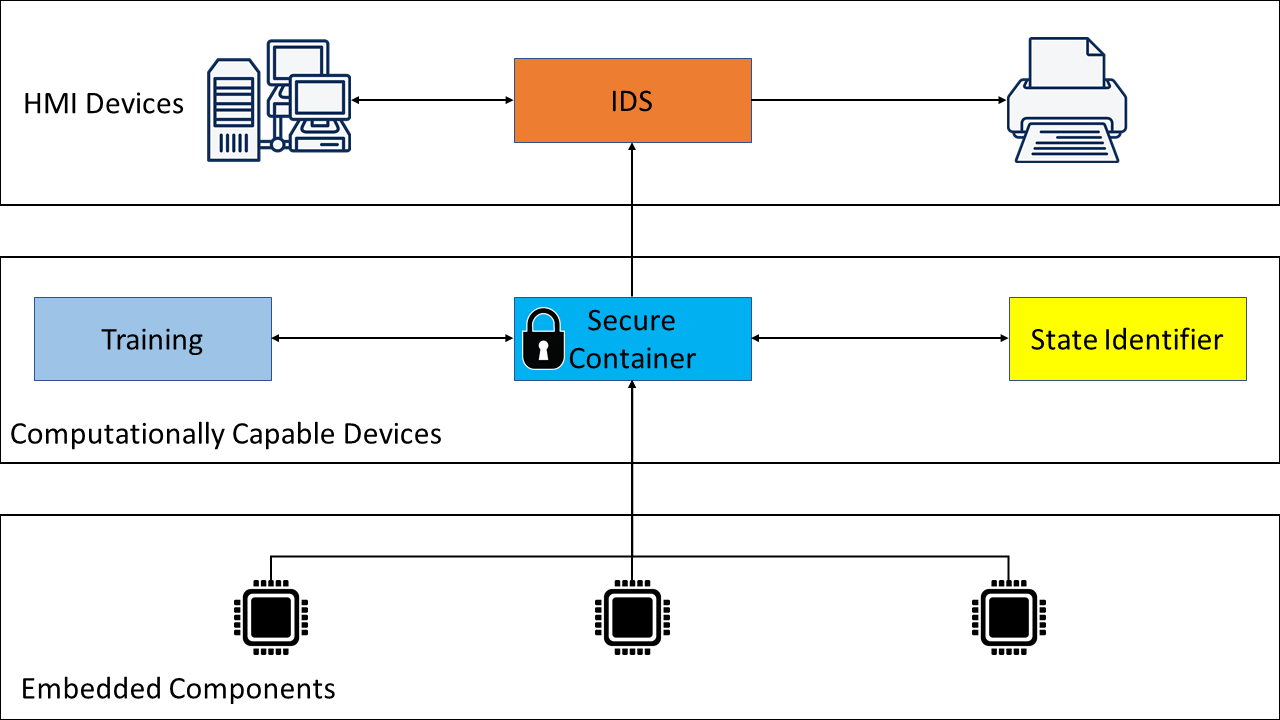
\includegraphics [width=.5\textwidth]{sec_scada.png}}
\caption{Components of Secure Industrial Control System }
\label{sec_ics}
\end{figure}

%%This node can perform security analysis to identify if the device is compromised.

\subsection{State Identification}
This system component of the architecture is responsible for identifying important information about the state of the device. This module uses the information stored in the SDC to produce an image that represents an instantaneous state of the system that may result in a change in the network transmissions of the device. 

\subsection{Secure Data Container}
Our proposed solution for data protection in transit and at rest with providing leakage detection, as well as role-based and attribute-based access control, relies on the {\em Secure Data Container} (SDC). The SDC concept was inspired by the Active Bundle  \cite{c12}, \cite{c13}, \cite{c14}, \cite{c15} and the Extended Attribute-Aware Active Bundle (EA3B) \cite{c6} concepts. The SDC is a self-protecting data container that incorporates data in encrypted form with watermarks, access control policies, metadata, and a policy and attribute enforcement kernel, as shown in Figure~\ref{sdc}. In addition to a Java\textsuperscript{\textregistered} Executable Archive (JAR), used in AB \cite{c14}, \cite{c15} and EA3B \cite{c6}, the SDC supports a spreadsheet implementation with encrypted worksheets. Thus, an SDC that stores log records as well as sensor data snapshots, provides an easier integration into existing IT infrastructures, compared to EA3B. Each separate data subset is stored as a separate worksheet in a spreadsheet file encrypted with separate AES key that is generated on-the-fly when a client requests data from an SDC. 

\begin{figure}[htbp]
\centering
\centerline{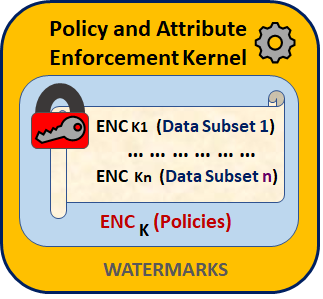
\includegraphics [width=4.5cm, height=4.3cm]
{SDC-Rel.png}}
\caption{Secure Data Container}
\label{sdc}
\end{figure}

The access control model relies on role-based and attribute-based access control and guarantees that a client is able to access only those data subsets from SDC for which the client is authorized. SDC provides tamper-resistance and data integrity. Unauthorized modification of policy evaluation code or access control policies leads to wrong decryption key derivation. Moreover, just as EA3B, SDC can detect several types of data leakages that can be made by authorized insiders \cite{c6}. Data leakage detection relies on watermarks, embedded into each data subset and SDC itself. \\ 
The proposed solution for data protection works in both centralized and decentralized peer-to-peer network architectures. A Central Authority is not required for data recipient’s key generation or for access control policy enforcement.

\subsection{Training}
The {\em training module} will execute off-line to train the system such that it learns what device state results in particular network behavior. It will also identify the state information which is most likely to make significant change in the network traffic. The information from the state identifying module is used here. The training module will be fed with data collected from the state collection component and data collected by sampling the network. Machine learning algorithms are used to model the relationship between device state and specific network traffic. A dataset that represents this relationship is created from the model and stored for future use by the IDS. The IDS can query this information to verify its alerts.

\subsection{Intrusion Detection Process}
In order to detect unusual network behavior that is not caused by an intrusion, the IDS in this component does not rely on network traffic alone. If an alert is generated from abnormal activity in the network, the IDS queries the information stored by the training module. The device state information related to the specific network data is used to verify the alert. This allows the IDS to reduce false positives. The IDS also receives real-time information from the state router and performs analysis to detect compromised device. 

\section{Evaluation}
Our initial evaluation includes experiments that show improved IDS results and the performance overhead of the SDC. To show improved IDS results, we used a dataset \cite{c7} created by the Mississippi State University SCADA Security Laboratory and Power and Energy Research laboratory, which is a collection of network data from a water storage tank system. The dataset is generated for performing intrusion detection to detect seven different attack scenarios.
\begin{figure}[htbp]
\centering
\centerline{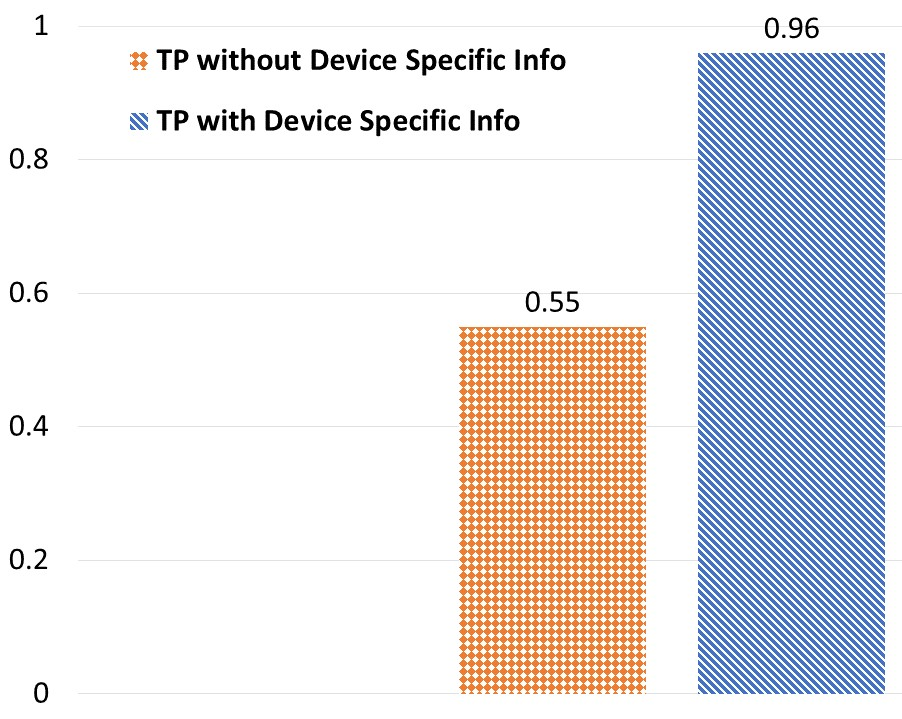
\includegraphics [width=.3\textwidth, height=4cm]{chart.jpg}}
\caption{TP Rate for Attack Detection in Water Storage Dataset}
\label{eval-anomaly}
\end{figure}
Based on the behavior of the process, the network trace was annotated with data representing device state for the network data it generated. We used the Naive Bayes algorithm to create a model with the new dataset. The added information increases the machine learning algorithm's true positive rate significantly (75\%). The comparison is shown in Figure ~\ref{eval-anomaly}.

To measure the performance overhead of the SDC, we collected data request Round-Trip Time (RTT) by measuring the time starting from a web service's data request to SDC and ending with the receipt of the response from SDC. RTT is a sum of times spent for authentication, evaluation of access control policies and the client’s attributes, decryption key derivation and data retrieval. The ApacheBench\textsuperscript{\textregistered} utility (version 2.3) and web browser developer consoles were used for RTT evaluations. A web service (client) requesting data, an authentication server, and the SDC are running on the same host to exclude network delays from RTT measurements. Experiments were conducted on two system configurations. \\ 
1. Hardware: MacBook\textsuperscript{\textregistered}\footnote{This is an independent publication and has not been authorized, sponsored, or otherwise approved by Apple Inc.} Pro, Intel\textsuperscript{\textregistered} Core i7 CPU @ 2.2 GHz, 16GB memory; OS: macOS\textsuperscript{\textregistered} Sierra 10.12.6. \\
2. Hardware: ARMv7\textsuperscript{\textregistered} Processor rev 4 @1.2GHz, RAM 1GB (Raspberry Pi\textsuperscript{\textregistered}\footnote{Raspberry Pi is a trademark of the Raspberry Pi Foundation} 3 Model B); OS: Raspbian GNU/Linux\textsuperscript{\textregistered}\footnote{Linux® is the registered trademark of Linus Torvalds in the U.S. and other countries.} 9.1 \\
In our experiments, RTT was measured as an average of 50 requests for 16 bytes of data for SDC with 4 and 8 access control policies - see Figure ~\ref{eval-sdc}.

\begin{figure}[htbp]
\centering
\centerline{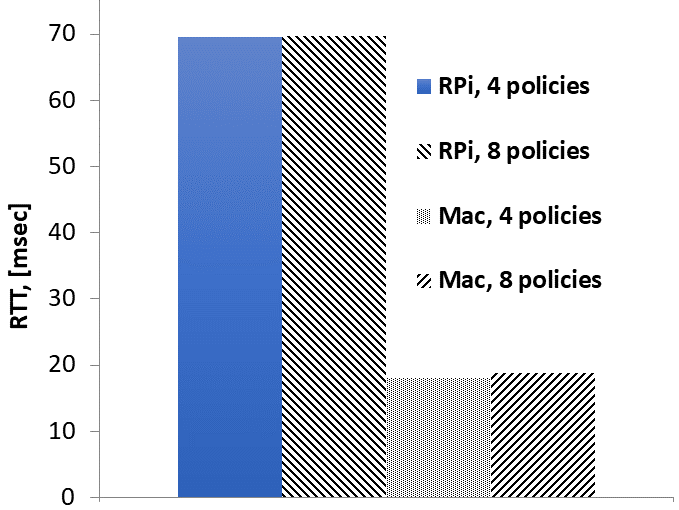
\includegraphics [width=.35\textwidth, height=4cm]{SDC-Eval-Plat-OK.png}}
\caption{SDC Data Request Round-Trip Time}
\label{eval-sdc}
\end{figure}

As it can be seen from Figure ~\ref{eval-sdc}, RTT strongly depends on hardware that hosts SDC, and slightly depends on number of access control policies in SDC. Typically, hardware on level 1 in the secure ICS architecture (see Figure ~\ref{SICSA}) has less computationally powerful hardware to host SDC than on levels 2 and 3. On level 1, represented as a Raspberry Pi, RTT increases by 284\% for 4 policies and by 270.2\% for 8 policies in SDC. When the number of access control policies in SDC is increased from 4 to 8, RTT increased by 0.23\% for Raspberry Pi and by 4\% for MacBook Pro.     

\section{Future Work}
We have implemented a framework for secure data transfer and storage that relies on secure data containers. We also have an experimental environment, which can be used to generate real-world log data. We did preliminary investigation on machine learning algorithms that can be used to detect important artifacts that are responsible for triggering network data. In the future, a dataset will be generated to represent the relationship between the network data and the important device state data. We also plan to determine how to incorporate learned behavior into the IDS to improve its results and to reduce false positives. Furthermore, we plan to expand secure data container capabilities to provide guarantees for provenance data integrity. We explore blockchain-based approaches for collecting and storing provenance data.   

\section{Conclusion}
In this paper, we presented a method to improve IDS true positive rate in ICS using extra information about device state. This extra information is securely stored and transferred to the IDS by employing secure data containers that protect log data and device state information in transit and at rest. We have proposed a system for securely collecting and transporting state data and machine learning techniques that use this data to improve IDS results. 


\begin{thebibliography}{00}
\bibitem{c1}Industrial Control Systems (ICS) Market 2018 Global Analysis, Industry Size, Share Leaders, Current Status by Major Key vendors and Trends by Forecast to 2023. [Online] https://www.marketwatch.com/press-release/industrial-control-systems-ics-market-2018-global-analysis-industry-size-share-leaders-current-status-by-major-key-vendors-and-trends-by-forecast-to-2023-2018-11-29. Last accessed: Nov.2019
\bibitem{c2}Morris, T., Vaughn, R., \& Dandass, Y. (2012). A retrofit network intrusion detection system for MODBUS RTU and ASCII industrial control systems. Proceedings of the Annual Hawaii International Conference on System Sciences, 2338–2345.
\bibitem{c3}Tsang, C. H., \& Kwong, S. (2005). Multi-agent intrusion detection system in industrial network using ant colony clustering approach and unsupervised feature extraction. Proceedings of the IEEE International Conference on Industrial Technology, 2005, 51–56.
\bibitem{c4}Carcano, A., Coletta, A., Guglielmi, M., Masera, M., Nai Fovino, I., \& Trombetta, A. (2011). A multidimensional critical state analysis for detecting intrusions in SCADA systems. IEEE Transactions on Industrial Informatics, 7(2), 179–186. 
\bibitem{c5}Kiss, I., Genge, B., Haller, P., \& Sebestyen, G. (2014). Data clustering-based anomaly detection in industrial control systems. Proceedings - 2014 IEEE 10th International Conference on Intelligent Computer Communication and Processing, ICCP 2014, 275–281.
\bibitem{c6} Ulybyshev, Denis A, (2019). "Data Protection in Transit and at Rest with Leakage Detection". Ph.D. Thesis, Purdue University.
\bibitem{c7}Morris, T. Srivastava, A., Reaves, B., Gao, W., Pavurapu, K., Reddi, R. A Control System Testbed to Validate Critical Infrastructure Protection Concepts. International Journal of Critical Infrastructure Protection (2011). Elseiver.
\bibitem{c8}Asmar Awad, R., Lopez, J., and Rogers M. (2019) Volatile Memory Extraction-Based Approach for Level 0-1 CPS Forensics. Accepted to 2019 IEEE International Symposium on Technologies for Homeland Security. 
\bibitem{c9}Gao, W., \& Morris, T. (2014). On Cyber Attacks and Signature Based Intrusion Detection for Modbus Based Industrial Control Systems. Journal of Digital Forensics, Security and Law, 9(1). 
\bibitem{c10}Ranchal, R., Bhargava, B., Angin, P., \& Othmane, L. B. (2018). Epics: A framework for enforcing security policies in composite web services. IEEE Transactions on Services Computing.
\bibitem{c11} Williams, T. J. (1994). The Purdue enterprise reference architecture. Computers in industry, 24(2-3), 141-158.
\bibitem{c12} Lilien, L., \& Bhargava, B. (2006). A scheme for privacy-preserving data dissemination. IEEE Transactions on Systems, Man, and Cybernetics-Part A: Systems and Humans, 36(3), 503-506.
\bibitem{c13} Othmane, Lotfi Ben, and Leszek Lilien (2009). "Protecting privacy of sensitive data dissemination using active bundles." In 2009 World Congress on Privacy, Security, Trust and the Management of e-Business, pp. 202-213, IEEE.
\bibitem{c14} Ranchal, Rohit (2015). "Cross-domain data dissemination and policy enforcement". Ph.D. Thesis, Purdue University.
\bibitem{c15} Ulybyshev, D., Bhargava, B., Villarreal-Vasquez, M., Alsalem, A. O., Steiner, D., Li, L., \& Ranchal, R. (2017). Privacy-preserving data dissemination in untrusted cloud. In 2017 IEEE 10th International Conference on Cloud Computing (CLOUD) (pp. 770-773). IEEE.

\end{thebibliography}
\vspace{12pt}
\end{document}
